\section{Spacetime Rig Optimization}
\label{section:spacetime}

%As we discussed in Section~\ref{sec:rig_opt}, our motion optimizaion in rig space is performed by minimizing the energy based on a skeletal motion distance.
%Although this results a successful inverse mapping, it is not practical enough to be used in production.
%In this section, we present constraints to get artist-friendly results.
%In this section, we present the details of spacetime optimization process which is based on a skeletal motion distance subject to the constraints derived from the %regularization of rig parameters, acceleration energy of rig parameters, relative body segment constraints, and rig parameter constraints.
In this section, we present the details of our spacetime optimization process discussed in Section~\ref{sec:rig_opt}.
The motion optimization in rig space is performed by minimizing the energy-based on a skeletal pose distance subject to the constraints derived from the regularization of rig parameters, acceleration energy of rig parameters, rig parameter constraint, and relative skeletal segment constraints.

%\begin{figure}[ht]
%  \centering
%  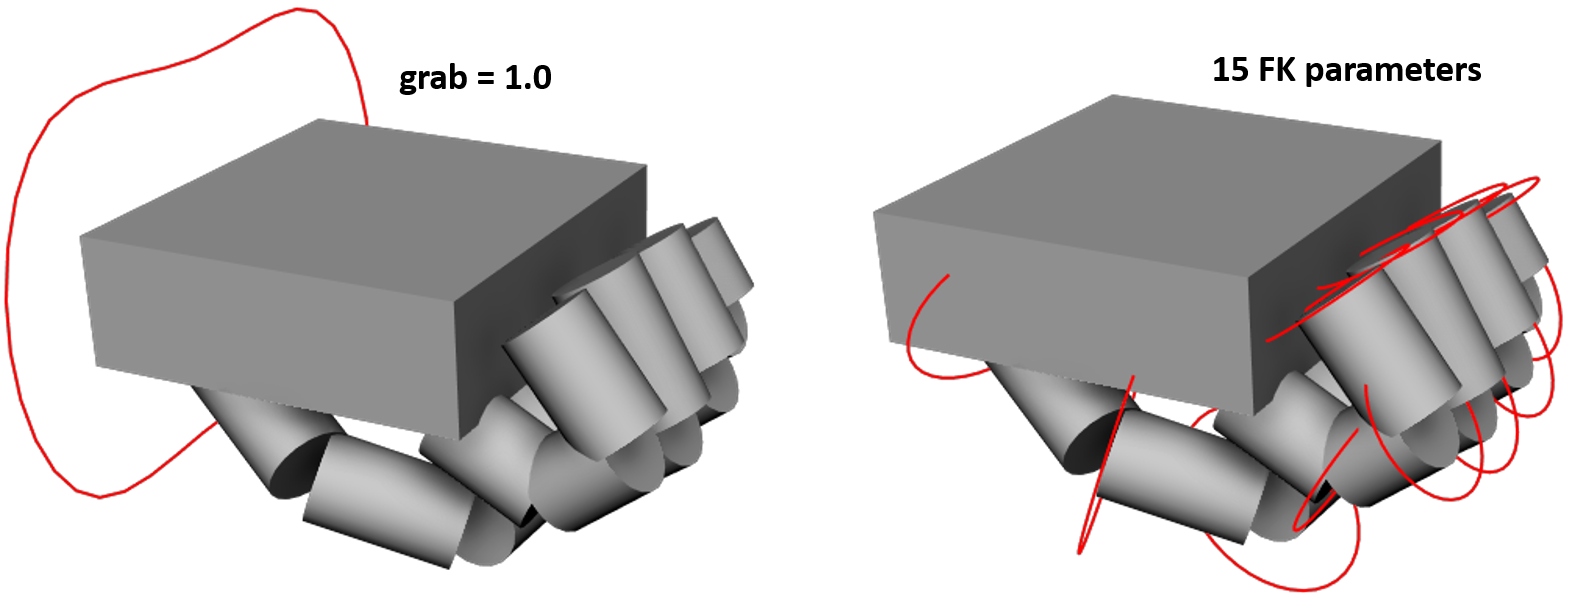
\includegraphics[width=3.0in]{images/handMultiSolution}
%  \caption{(a)Hand fist pose created by using one ‘grab’ parameter (b)Same pose created by using 15 FK parameters}
%  \label{fig:handRigExample}
%\end{figure}

%\begin{figure}[ht]
%  \centering
%  \begin{subfigure}[b]{0.20\textwidth}
%	  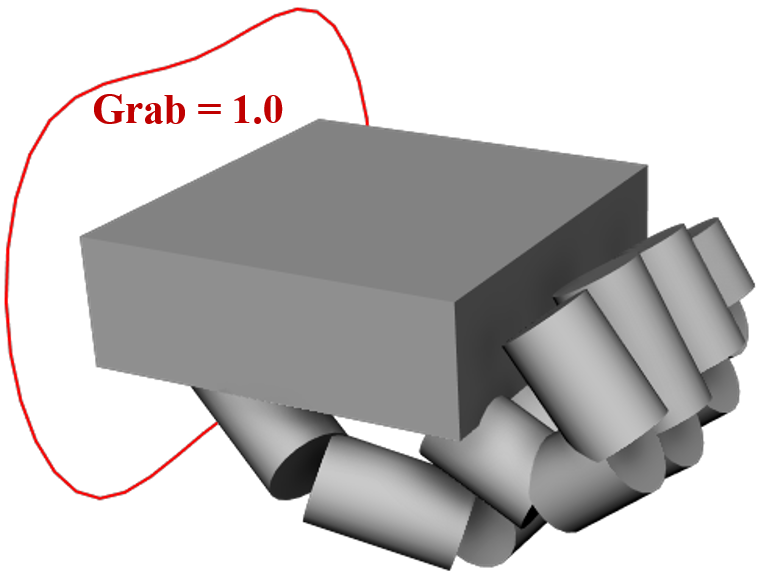
\includegraphics[width=3.0in]{images/grab}
%	  \caption{}
%	  \label{}
%  \end{subfigure}
%  \begin{subfigure}[b]{0.25\textwidth}
%	  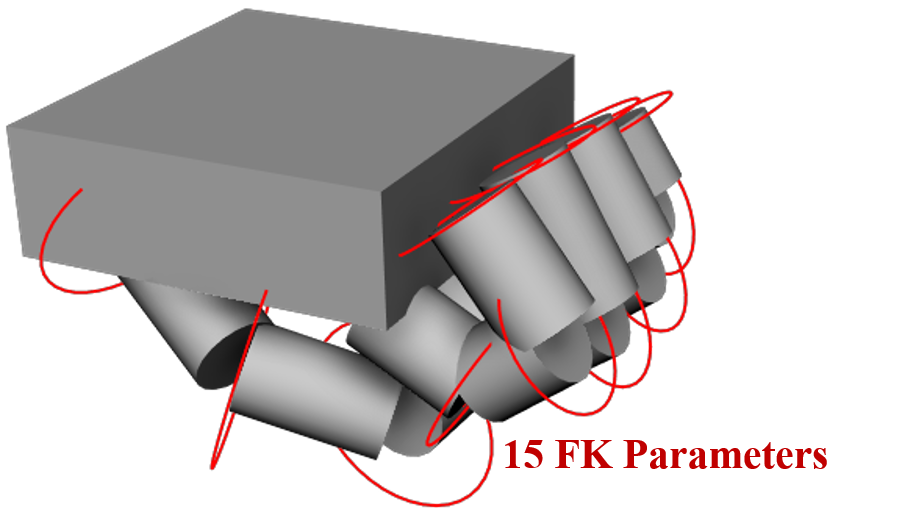
\includegraphics[width=3.0in]{images/fk15}
%	  \caption{}
%	  \label{}
%  \end{subfigure}
%  \caption{(a)Hand fist pose created by using one ‘grab’ parameter (b)Same pose created by using 15 FK parameters}
%  \label{fig:handRigExample}
%\end{figure}

\begin{figure}[!ht]
    \centering
    \begin{subfigure}[b]{0.2\textwidth}
        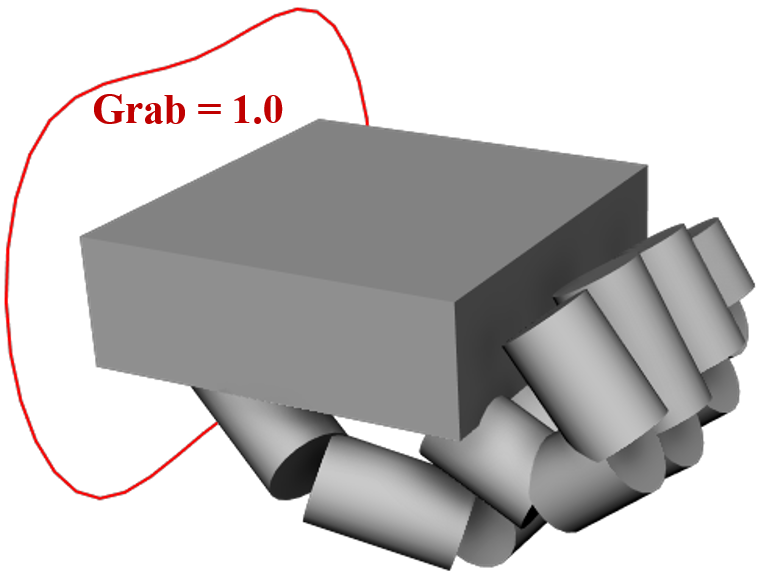
\includegraphics[width=\textwidth]{images/grab}
        \caption{}
        \label{}
    \end{subfigure}
    %add desired spacing between images, e. g. ~, \quad, \qquad, \hfill etc. 
      %(or a blank line to force the subfigure onto a new line)
    \begin{subfigure}[b]{0.23\textwidth}
        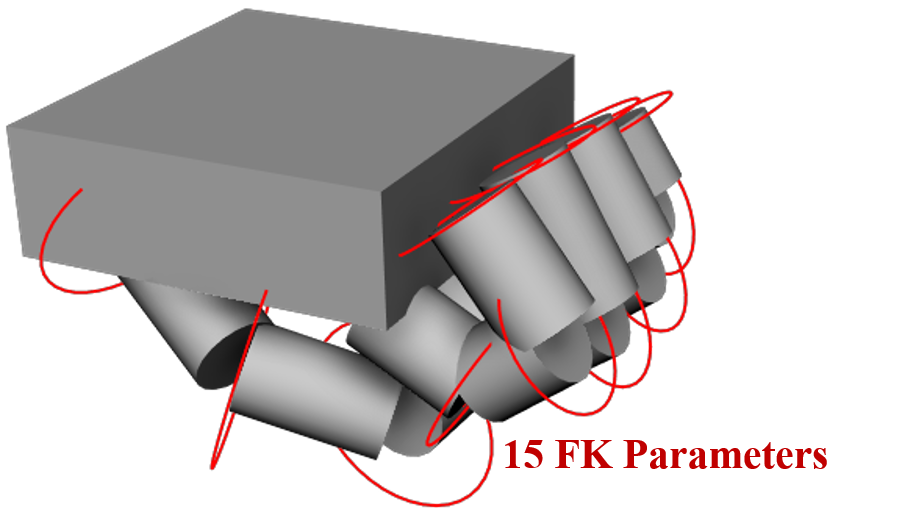
\includegraphics[width=\textwidth]{images/fk15}
        \caption{}
        \label{}
    \end{subfigure}
    
%    \begin{subfigure}[b]{0.45\textwidth}
%        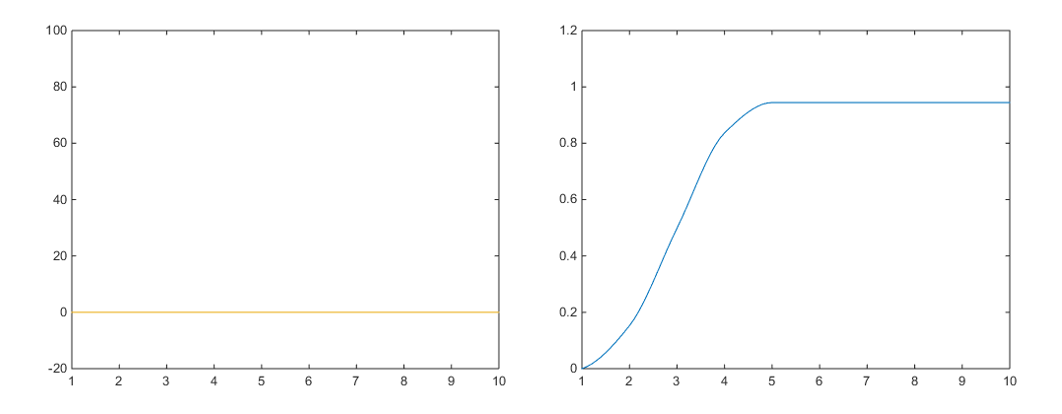
\includegraphics[width=\textwidth]{images/n1_big}
%        \caption{$\lambda = 1.0$}
%        \label{fig:reg_big}
%    \end{subfigure}
%    ~
%    \begin{subfigure}[b]{0.45\textwidth}
%        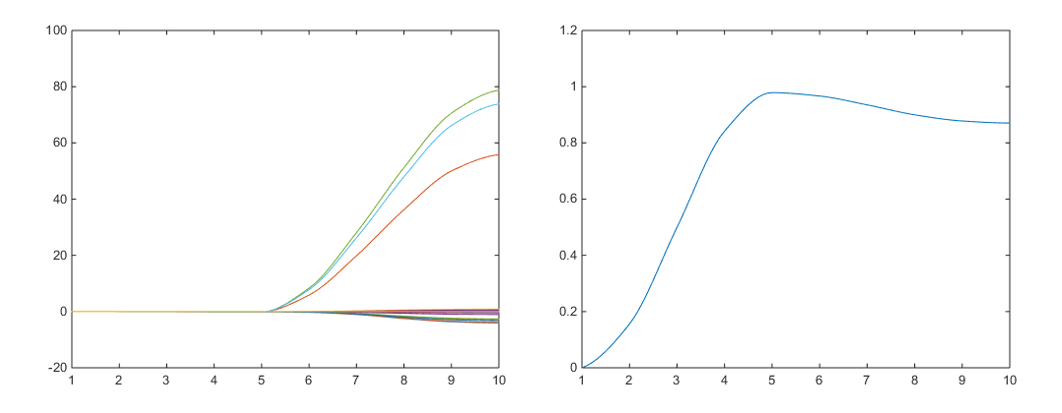
\includegraphics[width=\textwidth]{images/n1_small}
%        \caption{$\lambda = 0.0001$}
%        \label{fig:reg_small}
%    \end{subfigure}
    
    \caption{(a) Hand fist pose created by using one grab parameter (b) Same pose created by using 15 FK parameters
    }
    \label{fig:handRigExample}
\end{figure}


\textbf{Skeletal pose distance energy}
We illustrate the relationship between the skeletal pose $\mathbf{p}_i$ and its corresponding rig space parameter $\mathbf{c}_i$ in Section~\ref{sec:LigGroup}. Note that the solution of rig space parameter $\mathbf{c}_i$ for single pose $\mathbf{p}_i$ is not unique, in general. Figure~\ref{fig:handRigExample}(a) and (b) show that the same skeletal pose can be generated with different rig space parameters. In the animation production, the choice of rig space parameters is completely up to the preferences of the animator in such a case. Therefore, it is impossible to satisfy individual preference of the artist without any prior data. 
Instead, we define the optimality of the rig space parameters from the character rig functionality point of view. Riggers provide various functions to simplify the generation of complex motion with a small number of parameters\cite{orvalho2012facial}. In Figure~\ref{fig:handRigExample}, example (a) utilizes a custom parameter called \textit{grab} that activates on a single scalar value while example (b) relies on as many as 15 three dimensional \textit{FK} parameters. While the effects are same, the solution of example (a) is preferred over that of example (b) because it modifies fewer number of parameters. 
To reflect this, we choose the solution that involves a minimum number of parameters, when there are multiple solutions $\Delta{c(i)}$.
The energy term for the skeletal pose distance is represented as follows:

\begin{equation}
E_{p}(t) = \left \| \mathbf{J}(t)\Delta \mathbf{c}(t)-\Delta \mathfrak{p}(t) \right \|^{2}+\lambda \left | \Delta \mathbf{c}(t) \right |_1,
\end{equation}

where $\mathbf{J}$ is the Jacobian matrix of $\Delta \mathfrak{p}$ with respect to $\Delta\mathbf{c}$ at current time $t$, and $\lambda$ is the regularization weight parameter. The Jacobian matrix cannot be defined analytically because we do not assume any prior information about the exact function of each rig parameter. Therefore, we use approximate Jacobian obtained by finite differences of the current rig state. This process is known to be very slow\cite{hahn2012rig} because every rig parameter should be accessed to update the Jacobian. Fortunately, the Jacobian does not have to be recomputed in every iteration because when the rig skeletal pose approaches to the target pose, the Jacobian remains alomost the same. Our experiments show that the fine tuning of the pose requires more than 60\% of the computation time. Therefore, we reuse the same Jacobian from the previous iteration when the current pose distance is smaller than a threhshold $\eta$. Moreover, we already reduced the number of rig parameters in the rig analysis stage, thus we could enhance the performance of the Jacobian computation. The threshold $\eta$ is user parameter that depends on the number of skeletal segments and the global scale of the character. In our experiment, $\eta = 0.1$ showed reasonable results.
%We locally compute Jacobian matrix $\mathbf{J}$ at the current state and find $\Delta \mathbf{c}^*(t)$ to reach the target pose $\bar{\mathfrak{p}}(t)$ by performing the local linear approximation on the Lie algebra vector space. 
%\textbf{For faster computation time, we updated the $\mathbf{J}$ until the pose distance is under certain threshold, and used the same one until it converge.}

Note that we performed the L1 regularization on $\Delta{c}$. The L1 regularization favors a sparse solution of rig parameters and force the small weight parameters converge to 0. This allows to provide the animator with the minimum number of resulting parameters to deal with, for the creation of animation.
Our solution also satisfies the artist's preference toward sparse parameters in generating motions\cite{seol2011artist}. Although the optimal regularization weight $\lambda$ can be estimated through the cross-validation after the optimization, the value of $0.001$ achieved reasonable regularization for various rigs in our experiments.

\textbf{Acceleration energy}
Since we optimize rig space parameters for each pose, popping artifact may occur. To address this, we minimize the acceleration energy at time $t$, so that the rig space parameters change smoothly across adjacent frames:
\begin{equation}
E_{a}(t) = \frac{1}{2}\left \| \Delta C(t-1)-2\Delta C(t)+\Delta C(t+1) \right \|^{2}, \\
\end{equation}

\subsection{Constraints}

\textbf{Rig parameter constraint}
Although we provide the optimal solution from a rig functionality point of view, the artist may prefer a different solution depending on the situation. We introduce a rig parameter constraint $K_{anim}$ to incorporate the artist's preference in the optimization process. The rig parameter constraint provided by the artist is calculated as:

\begin{equation}
K_{anim} (t) = \mathbf{K}_{anim}(t) \Delta C(t) - \mathbf{h}_{anim},
\end{equation}

where $\mathbf{K}_{anim}$ is the system constraint matrix (See Appendix A for details), and $\mathbf{h}_{anim}$ is the constraint vector that pushes the rig parameter toward the value designated by the artist.

\textbf{Relative skeletal segment constraints}
Self-penetration is one of the frequently occurr errors that the artist has to fix after the mapping to the rig space. The self-penetration occurs in the vertex level and the mesh level collision detection is not considered in this paper. Instead, we let the artist specify relative distance constraints between the skeletal segments. The relative distance constraint is represented as relative transformations between the two skeletal segments. Therefore, the relative skeletal segment constraint $K_{rel}$ at time $t$ is defined as follows:

\begin{equation}
K_{rel} (t) = \mathbf{K}_{rel}(t) \Delta C(t) - \mathbf{o}_{rel},
\end{equation}

where $\mathbf{K}_{rel}$ is the Jacobian matrix that represents how the relative transformation between the two body segments are changed by rig space parameter $\Delta C(t)$. $\mathbf{o}_{rel}$ represents the pose distance from current rig segments pose to desired pose given by the artist. Although our optimization is performed separately for each rig group, the relative distance constraint can be applied to any skeletal segment. For example, even if the arm and the spine of a human character is divided into two different groups, the constraint can be applied to prevent the two segments from colliding with each other.

%\textbf{Constraint energy}
%
%\begin{equation}
%\begin{split}
%E_{k} = \frac{1}{2} \Delta C^{T}\mathbf{K}^{T}\mathbf{W}\mathbf{K}\Delta C - \mathbf{k}^{T}\mathbf{W}\mathbf{k} +
%\frac{1}{2}\mathbf{k}^{T}\mathbf{W}\mathbf{k}
%\end{split}
%\end{equation}
%where $W$ is weight matrix that the purpose is assigning different weight to each constraint.

\subsection{Iterative optimization} \label{objectiveFunction}
We defined the relative skeletal segment constraint as a soft constraint, and the rig parameter constraint as a hard constriant.
Denoting the soft constraint as $E_s$ and the hard constraint as $E_h$, the objective function can be represented as follows:

\newcommand{\argmin}{\operatornamewithlimits{argmin}}

\begin{equation}
\argmin_{\Delta{\mathbf{c}(t)}}{\sum_t^n \left( {E_p(t) + w_aE_a(t)+E_s(t)+ \mathbf{z}^T E_h}\right)},
\label{eq:objectiveFtn}
\end{equation}

where $n$ indicates the number of frames, $w_a$ is the weight for the acceleration energy, and $\mathbf{z}$ denotes the Lagrange multipliers. $E_a$ at the first and the last frame is zero. Eq.~\ref{eq:objectiveFtn} can be rewritten in a matrix form as follows:
\begin{equation}
\begin{split}
\begin{bmatrix}
\boldsymbol{J}^T\boldsymbol{J}+w_a\boldsymbol{A}^T\boldsymbol{A}+\boldsymbol{K}_s^T\boldsymbol{W}\boldsymbol{K}_s+\boldsymbol{L} & \boldsymbol{K}_h^T\\ 
\boldsymbol{K}_h & 0 
\end{bmatrix}
\begin{bmatrix}
\Delta\boldsymbol{C}\\ 
\boldsymbol{Z}
\end{bmatrix}\\
=
\begin{bmatrix}
\boldsymbol{J}^T\Delta\boldsymbol{S} + \boldsymbol{K}_s^T\boldsymbol{W}\boldsymbol{k}_s\\ 
\boldsymbol{H}
\end{bmatrix},
\end{split}
\end{equation}

where $\boldsymbol{J}$, $\boldsymbol{K_s}$, $\boldsymbol{K_h}$ are diagonalized block matrices in time t of $\mathbf{J}$, $\mathbf{K_{anim}}$, $\mathbf{K_{rel}}$, respectively, $\Delta\boldsymbol{C}$, $\boldsymbol{Z}$, $\Delta\boldsymbol{S}$ and $\Delta\boldsymbol{H}$ are concatenated vector in time t of $\Delta\mathbf{c}$, $\Delta\mathbf{z}$, $\Delta\mathbf{s}$ and $\Delta\mathbf{h}$ respectively, and $\boldsymbol{W}$ is weight matrix for $\boldsymbol{K_s}$. $\boldsymbol{L}$ and $\boldsymbol{A}$ are the regularization matrix and the acceleration energy matrix, respectively\cite{ho2010spatial}.(See Appendix A for full details)
%$\boldsymbol{L}$ is regularization constraint matrix, and $\boldsymbol{A}$ is accereleration energy matrix where each is explained in Appendix.
The optimization terminates if it reaches the maximum iteration number $max_i$ or the magnitude difference of the rig space parameter $||\Delta c(t)||^2$ between the iteration steps is below a certain threshold $\epsilon$. 

%Since the each body segment group is independent, the order of optimization each group is irrelevant. 

%Our optimization is performed iteratively at every timestep(frame) $t$.

%Here, we set the user parameter $(max_i, \epsilon)$ as $(100, 10^{-100})$.
%Note our results are optimized in order of hierarchy of skeleton structure.